\documentclass[a4paper]{article}

\usepackage[toc,page]{appendix}

\usepackage[spanish]{babel}
\usepackage[utf8]{inputenc}
\usepackage{amsmath}
\usepackage{graphicx}
\usepackage{fancyhdr}
\usepackage{amsmath}
\usepackage[colorinlistoftodos]{todonotes}
\usepackage{xcolor}
\usepackage{minted}
\usepackage[font=small,labelfont=bf]{caption}
\usepackage{enumitem}
\usepackage{textcomp}
\usepackage{siunitx}
\usepackage{textgreek}
\usepackage{bigints}
\usepackage{amsfonts}

\usepackage{hyperref}

\hypersetup{
    colorlinks,
    citecolor=blue,
    filecolor=blue,
    linkcolor=blue,
    urlcolor=blue
}

\usepackage{geometry}
\geometry{a4paper}

\begin{document}
\begin{figure}
\centering
\includegraphics[scale=1]{./img/logo-facu}
\end{figure}

\title{\large\textsc{66.61 - Tecnología de Circuitos Integrados}\\
\large Trabajo Práctico Final\\
Sintetizador de Frecuencias para un Microcontrolador con un PLL Digital}

\author{
Andrew Parlane \\
}

\maketitle

\newpage

\tableofcontents

\listoffigures

\newpage

\section{Objetivo}

El objetivo de este trabajo es diseñar un sintetizador de frecuencias para uso en un microcontrolador con un PLL digital. Debería tomar un reloj de entrada con frecuencia $f_{ref}$ y unas señales de control y producir un reloj de salida con frecuencia $f_{o} = N f_{ref} / M$, donde N y M depende en las señales de control.

\section{TSMC 180}

Para comenzar tuve que aprender un poco sobre la tecnologia de TSMC 180. Leyendo los documentos dados encontré:

\begin{tabular}{l r}
    Parámetro & Valor \\ \hline
    $L_{MIN}$ & \SI{0.18}{\micro\meter} \\
    $W_{MIN}$ & \SI{0.42}{\micro\meter} \\
    $LD_{MIN}$ & \SI{0.48}{\micro\meter} \\
    $V_{DD_{MAX}}$ & \SI{1.8}{\volt} \\
\end{tabular}

No pude encontrar una lista de capacitancias entre cada capa, pero en el spice.lib encontré $t_{OX} = \SI{4.1}{\nano\meter}$, con esto pude calcular $C\prime_{OX} = \SI[per-mode=symbol]{8418}{\atto\farad\per\micro\meter\squared}$.

Realicé una simulación para encontrar el mejor ratio entre $W_N$ y $W_P$. Figura \ref{fig:wpfact_sch} muestra el esquemático y Figura \ref{fig:wpfact_sim} muestra el resultado. El mejor tiempo de propagación es dado cuando $W_P = 1.5 W_N$. Así en este proyecto uso WPFACT = 1.5.

\begin{figure}[!htb]
\centering
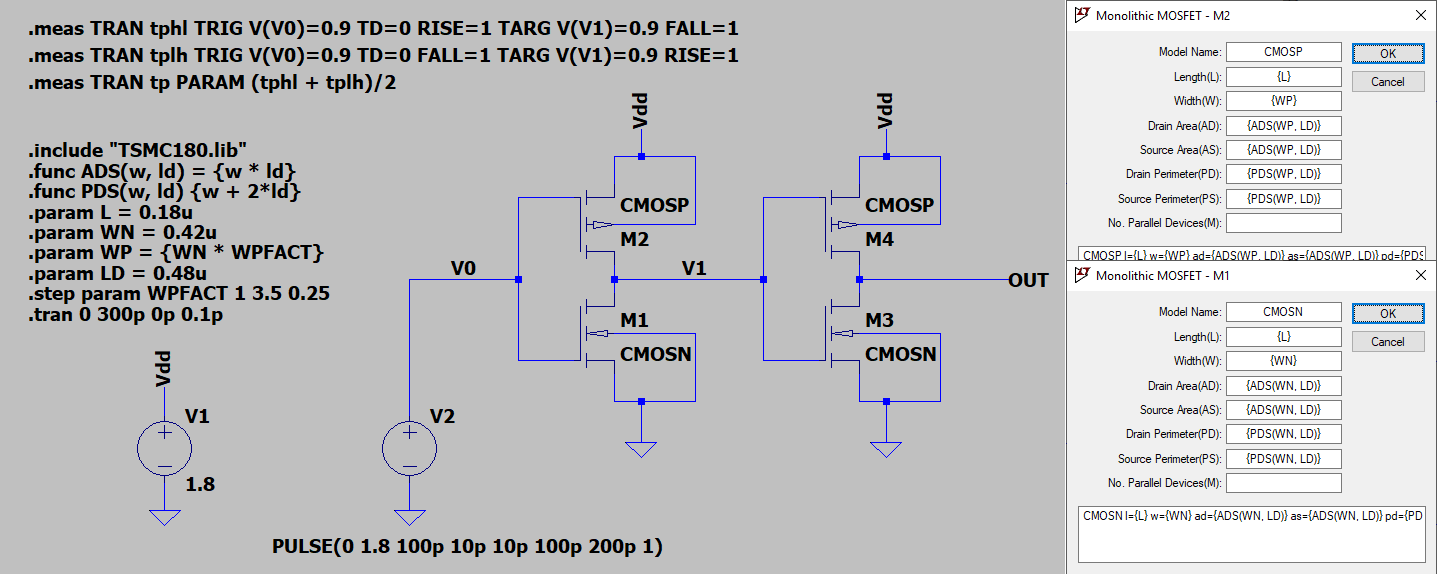
\includegraphics[scale=0.3]{./img/wpfact_sch}
\caption{Esquemático de dos inversores cascadas.}
\label{fig:wpfact_sch}
\end{figure}

\begin{figure}[!htb]
\centering
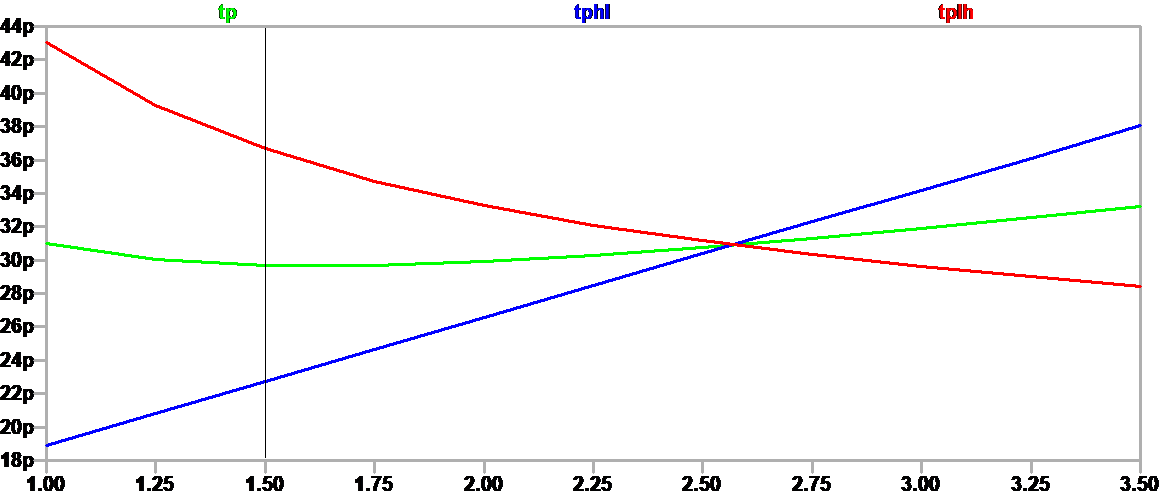
\includegraphics[scale=0.4]{./img/wpfact_sim}
\caption{Simulación para encontrar el mejor ratio entre $W_N$ Y $W_P$}
\label{fig:wpfact_sim}
\end{figure}

\section{Compuertas básicos}

Implementé varias compuertas básicos y realicé simulaciones para verificar su comportamiento. Los componentes que diseñe son:

\begin{itemize}[noitemsep]
    \item AND con 2, 3 y 4 entradas.
    \item FFD con reset asincróno.
    \item Inversor con el drain conectado a $V_{DD}$ y el source conectado a tierra.
    \item Inversor con el drain y el source exportado en el netlist.
    \item MUX con 2 vias.
    \item MUX con 4 vias y salida invertido.
    \item NAND con 2, 3 y 4 entradas.
    \item NOR con 2 entradas.
    \item OR con 2 entradas.
    \item Transmission Gate.
    \item XNOR con 2 entradas.
    \item XOR con 2 entradas.
\end{itemize}

No he usado todos en mi diseño final. Cada compuerta consiste de un .asc y un .asy, y es parametrizado así que cada instancia puede usar tamaños diferentes. Figura \ref{fig:compuertas_sch} muestra una selección de las compuertas.

\begin{figure}[!htb]
\centering
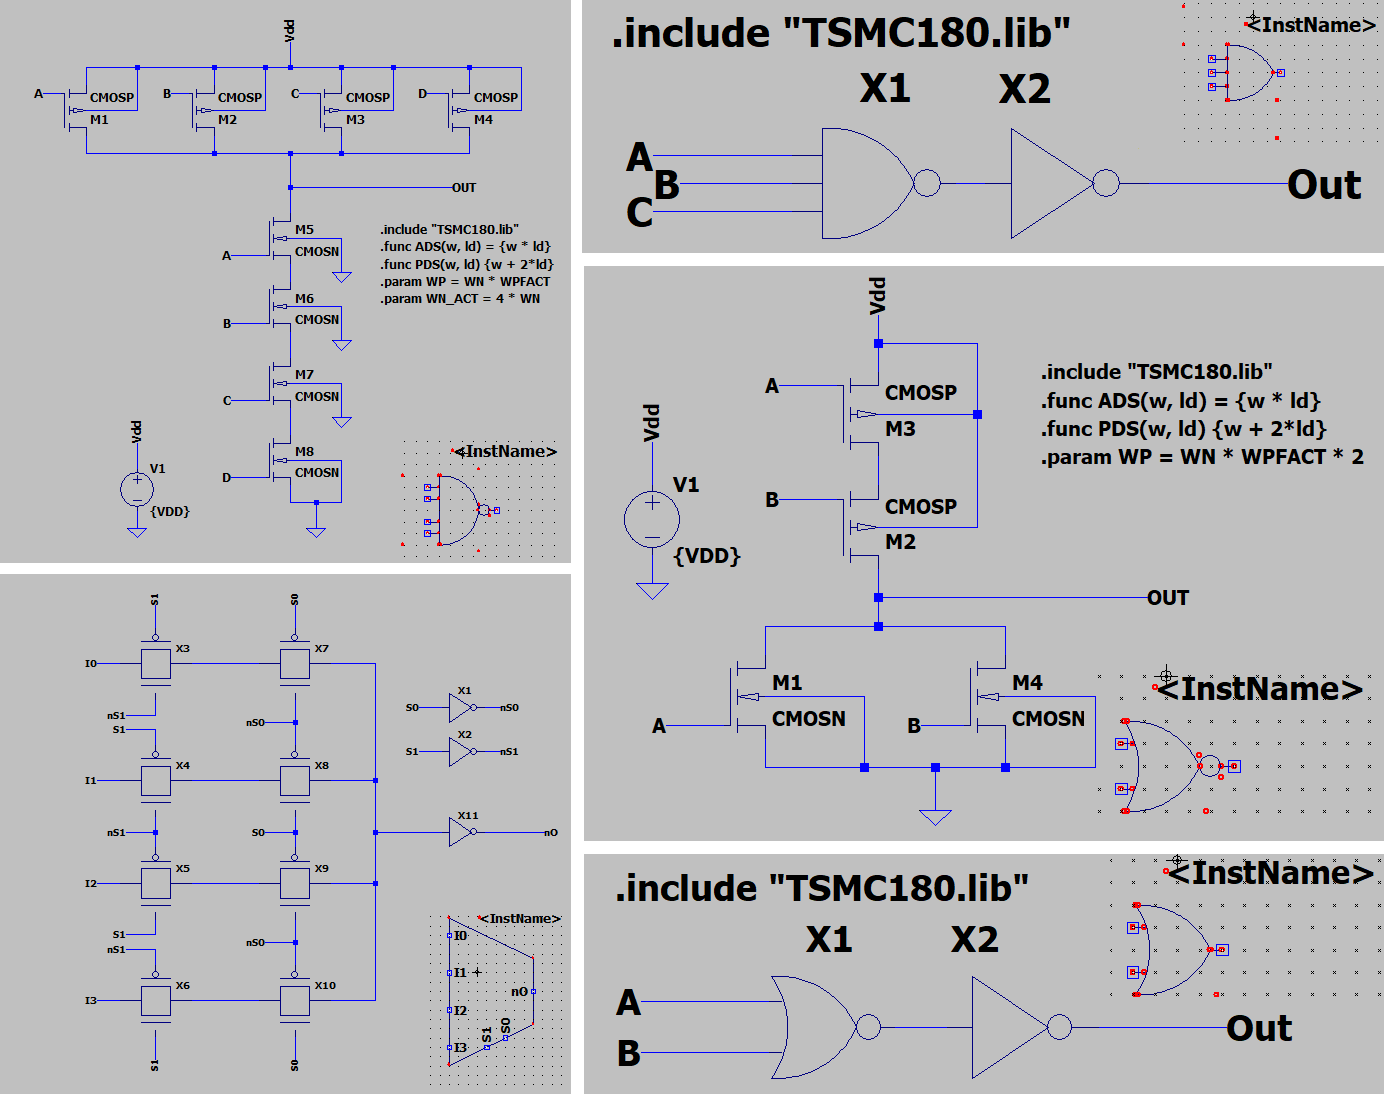
\includegraphics[scale=0.4]{./img/compuertas_sch}
\caption{Una selección de compuertas.}
\label{fig:compuertas_sch}
\end{figure}

\section{VCO}

Hay varias formas construir un VCO (por Voltage Controlled Oscillator), elegí usar un oscilador en anillo limitado por corriente. Figura \ref{fig:csro1} muestra la idea. Funciona cómo un oscilador en anillo normal pero los fuentes de corrientes controlan el tiempo de propagación del inversor, cambiando la frecuencia de operación:

\begin{align*}
C_{tot} &= \frac{5}{2} C\prime_{OX}(W_N L_N + W_P L_P) \\
f &= \frac{I_D}{N C_{tot} V_{DD}}
\end{align*}

Donde N es el número de inversores en el anillo, y $W_N, L_N, W_P, L_P$ son los anchos y largos de los transistores en los inversores. Elegí una corriente central de \SI{10}{\micro\ampere} que me da por inversores mínimos, y $N = 7$:

\begin{align*}
C_{tot} &= \SI{4.0}{\femto\farad} \\
f &= \SI{198.4}{\mega\hertz}
\end{align*}

\begin{figure}[!htb]
\centering
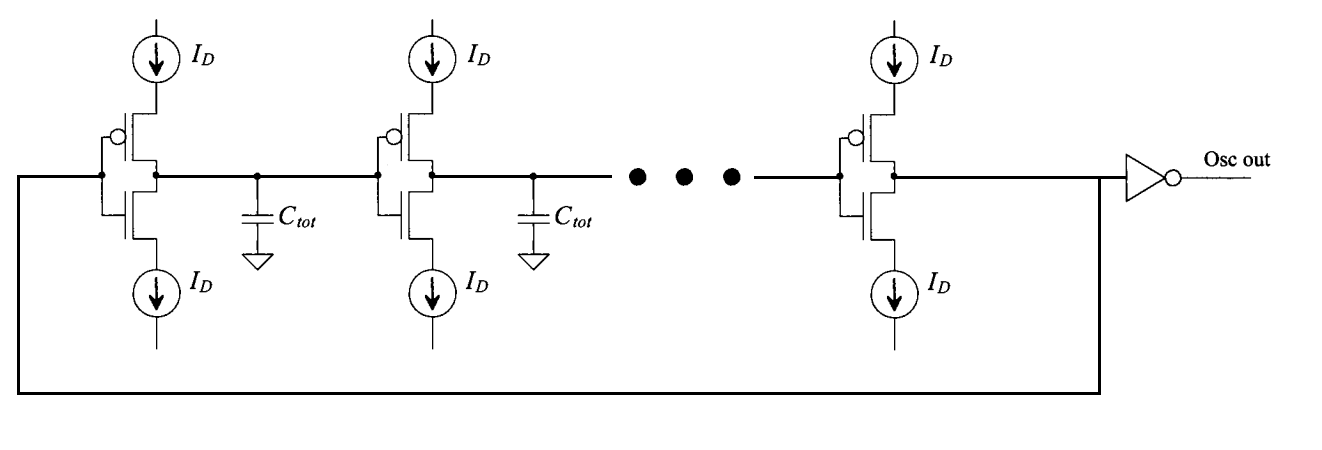
\includegraphics[scale=0.4]{./img/csro1}
\caption{Un Oscilador en Anillo limitado por corriente.}
\label{fig:csro1}
\end{figure}

El primer parte estuvo diseñar una fuente de corriente controlado por tensión. Figura \ref{fig:current_source_sch} muestra el diseño que usé.

\begin{figure}[!htb]
\centering
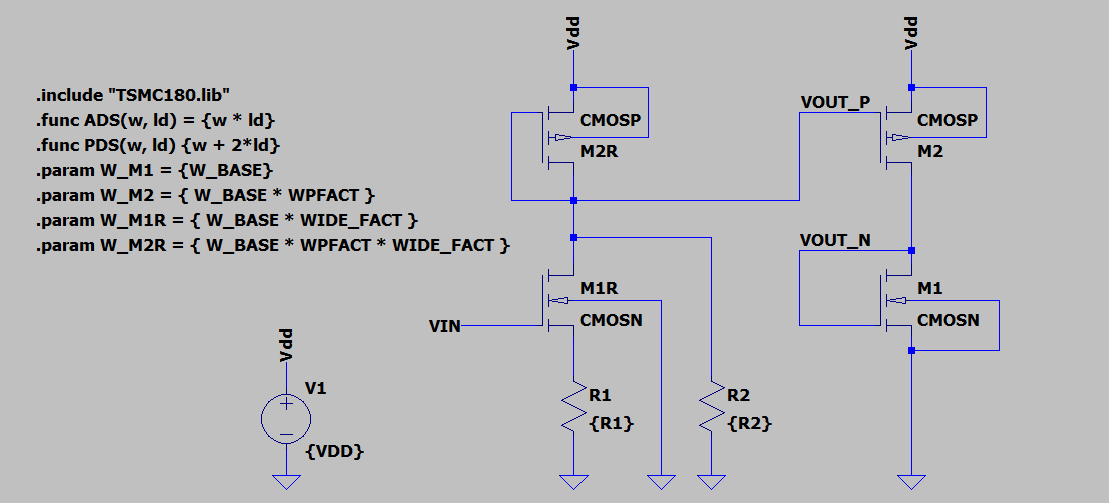
\includegraphics[scale=0.4]{./img/current_source_sch}
\caption{Fuente de corriente controlado por tensión.}
\label{fig:current_source_sch}
\end{figure}

El resistor R1 controla el pendiente de corriente contra tensión de $V_{IN}$. El resistor R2 controla el corriente mínimo cuándo $V_{IN} < V_T$, y los ratios de anchos de los cuatros transistores linearizan la salida.

Después de jugando con las simulaciones encontré los siguiente valores:

\begin{align*}
L &= \SI{0.9}{\micro\meter} \\
W_N &= \SI{4.0}{\micro\meter} \\
WPFACT &= 1.5 \\
WIDE_FACT &= 3 \\
R1 &= \SI{20.0}{\kilo\ohm} \\
R2 &= \SI{86.0}{\kilo\ohm}
\end{align*}

Que me da la salida mostrado en figura \ref{fig:current_source_sim}. Un corriente mínimo de \SI{5.0}{\micro\ampere}, un corriente central de \SI{9.9}{\micro\ampere}, y un corriente máximo de \SI{20.4}{\micro\ampere}. El pendiente es bastante lineal por $V_{IN} > \SI{0.7}{\volt}$, cómo mostrado con la línea azul, con una ecuación de $ I_D = \SI[per-mode=symbol]{11.5}{\micro\ampere\per\volt} V_{IN} - \SI{0.5}{\micro\ampere} $.

\begin{figure}[!htb]
\centering
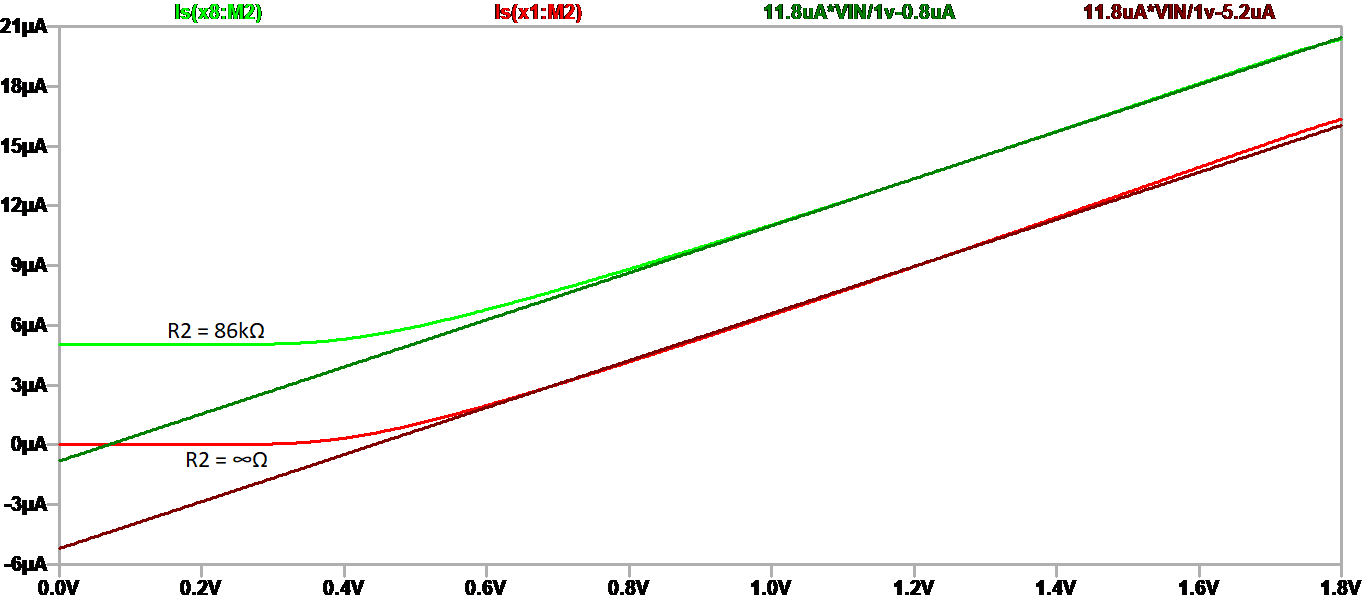
\includegraphics[scale=0.4]{./img/current_source_sim}
\caption{Simulación de la fuente de corriente controlado por tensión.}
\label{fig:current_source_sim}
\end{figure}

Figura \ref{fig:vco7_sch} muestra el esquemático del VCO, y Figura \ref{fig:vco7_test_sch} muestra el esquemático de prueba con todos los parámetros. Uso directivos de SPICE para medir y calcular la frecuencia promedio y el duty cycle sobre 100 ciclos. También calculo la frecuencia de salida esperado usando las ecuaciones anteriores. Encontré que la práctica y la teoría están bastante diferentes para inversores mínimos, así realicé otras simulaciones para ver cómo cambiando $W_N$ afecta estos valores. Figura \ref{fig:vco7_sim_wn} muestra el resultado. La frecuencia calculada y medida están iguales por $W_N = \SI{0.52}{\micro\meter}$ y $V_{IN} = \SI{0.9}{\volt}$. Intenté usar este valor pero la simulación estuvo dando me resultados raros por $V_{IN} < \SI{0.5}{\volt}$, así estoy usando $W_N = \SI{0.57}{\micro\meter}$.

\begin{figure}[!htb]
\centering
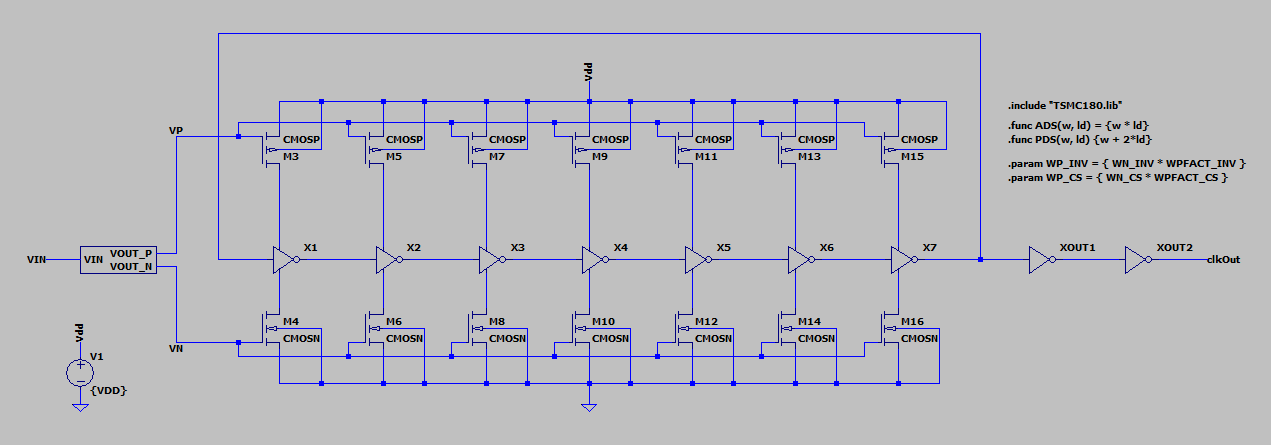
\includegraphics[scale=0.4]{./img/vco7_sch}
\caption{Esquemático del VCO.}
\label{fig:vco7_sch}
\end{figure}

\begin{figure}[!htb]
\centering
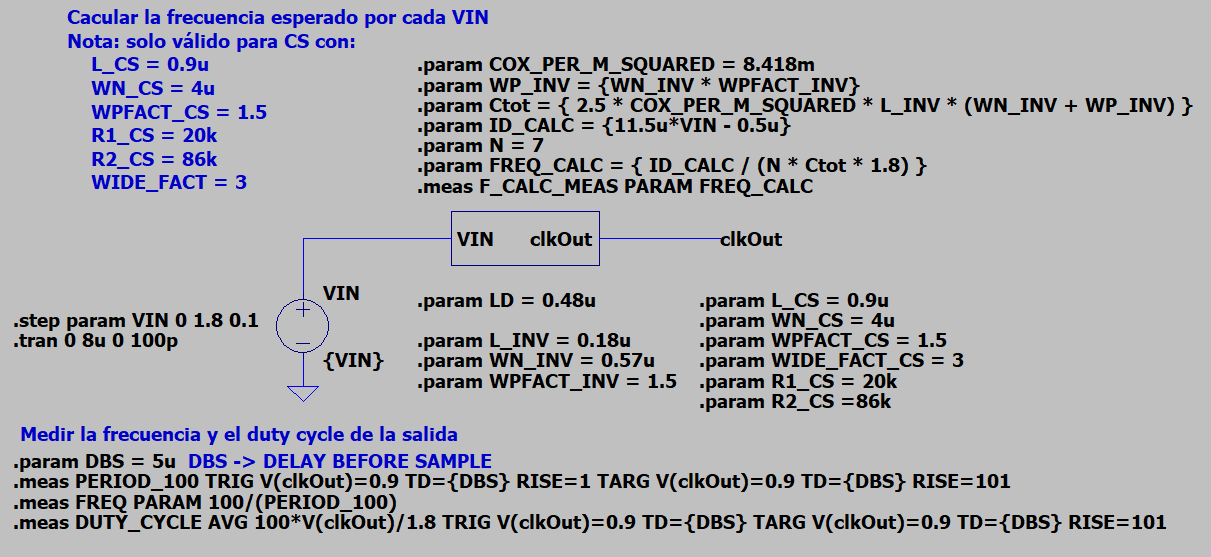
\includegraphics[scale=0.4]{./img/vco7_test_sch}
\caption{Esquemático de la prueba para VCO.}
\label{fig:vco7_test_sch}
\end{figure}

\begin{figure}[!htb]
\centering
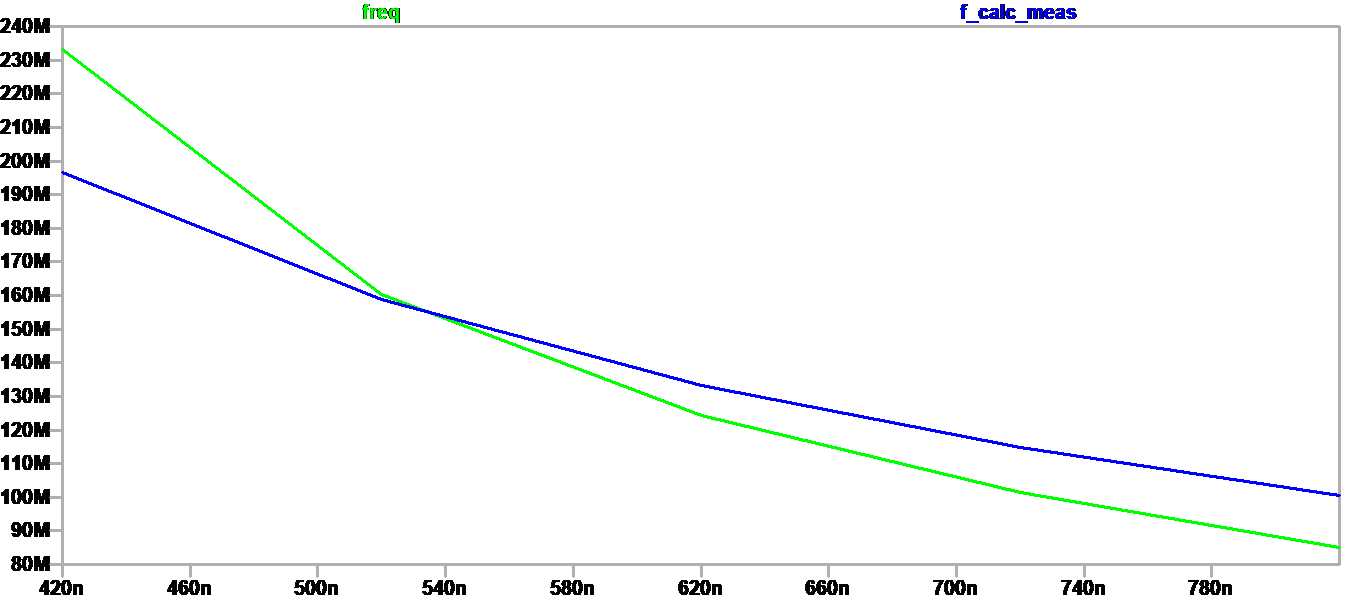
\includegraphics[scale=0.4]{./img/vco7_sim_wn}
\caption{Simulación de Frecuencia medida y estimada contra $W_N$.}
\label{fig:vco7_sim_wn}
\end{figure}

Figura \ref{fig:vco7_sim} muestra cómo cambia la frecuencia medido y estimado con $V_{IN}$. No están iguales pero están bastante cerca. El pendiente del parte lineal es aproximadamente \SI[per-mode=symbol]{200}{\mega\hertz\per\volt} dando un $K_{VCO} = 2\pi \cdot \SI[per-mode=symbol]{200}{\mega\hertz\per\volt} = \SI[per-mode=symbol]{1.26e9}{\radian\per\volt\per\second}$.

\begin{figure}[!htb]
\centering
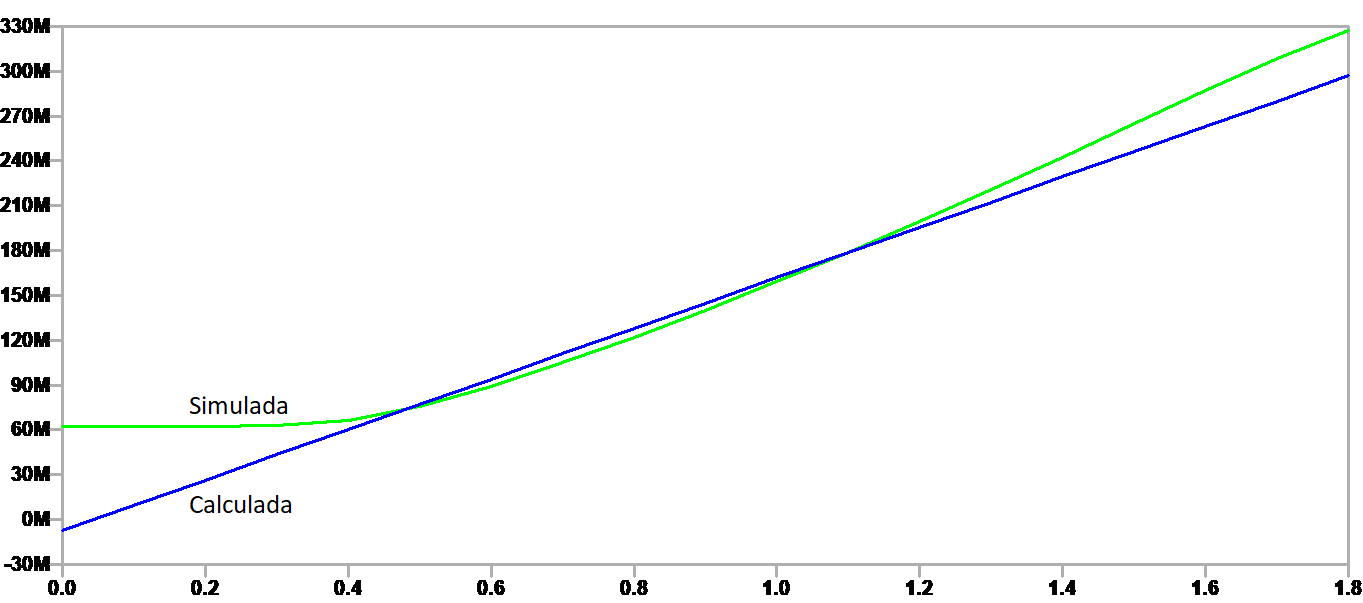
\includegraphics[scale=0.4]{./img/vco7_sim}
\caption{Simulación de Frecuencia medida y estimada contra $V_{IN}$.}
\label{fig:vco7_sim}
\end{figure}

\section{Divisor de Frecuencias}

Hay varias arquitecturas para implementar divisores de frecuencias, cual es mejor depende en la especificación del proyecto. Para este trabajo quise dividir por un valor programable.

Al principio implemente un divisor de frecuencias que puede dividir por $2^N$. La implementación es N FFDs en cascada cómo muestra Figura \ref{fig:freq_div_power_2_sch}. Cada ciclo del clkIn hace que div2 invierte su valor, así div2 completa un ciclo cada dos ciclos de/ clkIn. Después div4 completa un ciclo cada dos ciclos de/ div2, o cuatro ciclos del clkIn, etc... Mi implementación solo permite dividir hasta 16, para dividir por factores más altos puede conectar dos de los componentes en cascada. Un MUX puede ser usado para elegir la salida querido, como muestra Figura \ref{fig:freq_div_power_2_test_sch}.

\begin{figure}[!htb]
\centering
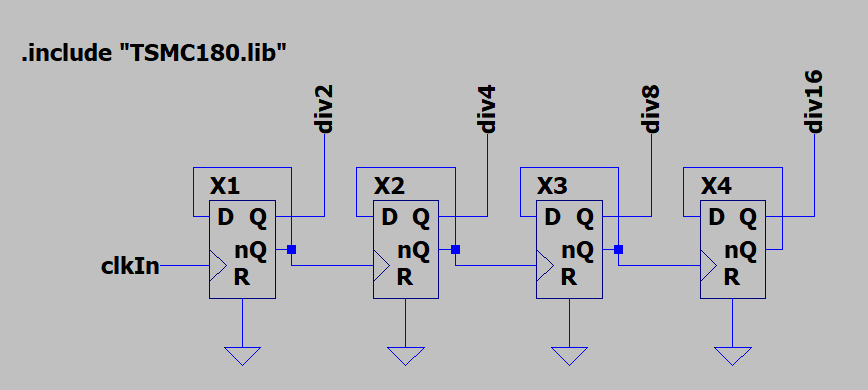
\includegraphics[scale=0.4]{./img/freq_div_power_2_sch}
\caption{Implementación de un divisor de frecuencias de $2^N$ }
\label{fig:freq_div_power_2_sch}
\end{figure}

\begin{figure}[!htb]
\centering
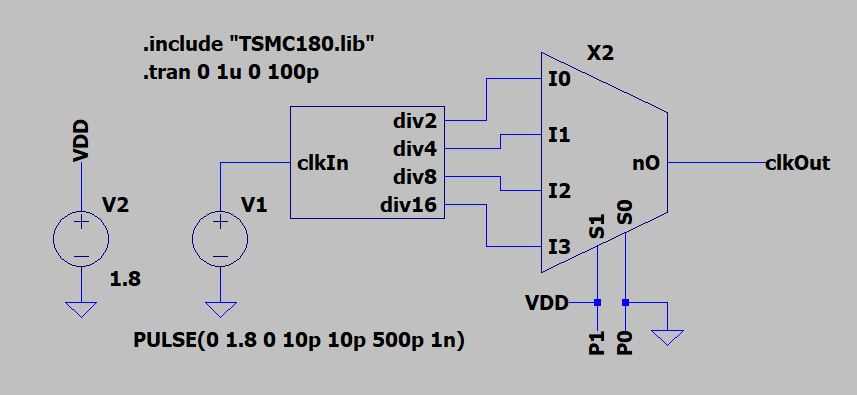
\includegraphics[scale=0.4]{./img/freq_div_power_2_test_sch}
\caption{Prueba para el divisor de frecuencias de $2^N$ }
\label{fig:freq_div_power_2_test_sch}
\end{figure}

El problema con esta arquitectura es que cuando está usado en el PLLD, solo se permite obtener uno o dos frecuencias válidos. Por ejemplo con el VCO descripto en la sección anterior, la salida del VCO tiene que ser entre \SI{60}{\mega\hertz} y \SI{330}{\mega\hertz}. Por un reloj de entrada de \SI{12}{\mega\hertz} solo podríamos usar un divisor de 8 para obtener \SI{96}{\mega\hertz} o de 16 para obtener \SI{192}{\mega\hertz}. Un divisor de 4 da una salida de \SI{48}{\mega\hertz} y un divisor de 32 da una salida de \SI{384}{\mega\hertz}, ambos de los dos están afuera del rango de la operación del VCO.

Un divisor que puede producir un rango lineal de salidas nos da más opciones. Así implementé un componente que divide por $2N$. Figura \ref{fig:freq_div_2n_sch} muestra una implementación. De nuevo usa una cadena de FFDs, pero este vez se usa como un contador digital. Unas compuertas XNOR hacen una comparación entre el valor del contador Q y el factor de división querido P. Cuando todos los bits están iguales invierte el clkOut. También implementé un otro divisor, mostrado en Figura \ref{fig:freq_div_2n_v2_sch}, que es muy parecido. La única diferencia es el comparador. Figura \ref{fig:freq_div_2n_test_v1_vs_v2_sim} muestra una simulación comparando los dos. El primer diseño (con las compuertas XNOR) es aproximadamente \SI{270}{\pico\second} más rápido que el segundo, así elegí usar eso. Los dos diseños no funcionan cuando $P = 0$ y dan una salida con frecuencia $f_{out} = f_{in} / 2P$ por los demás valores de P.

\begin{figure}[!htb]
\centering
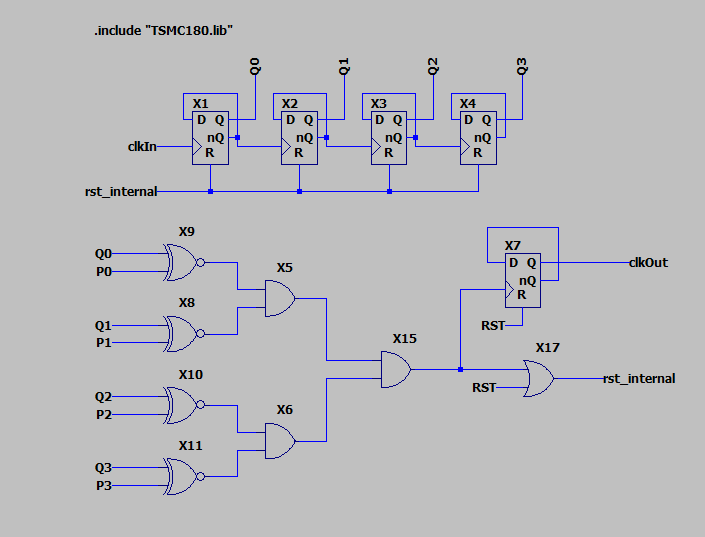
\includegraphics[scale=0.4]{./img/freq_div_2n_sch}
\caption{Divisor de frecuencias de $2N$. }
\label{fig:freq_div_2n_sch}
\end{figure}

\begin{figure}[!htb]
\centering
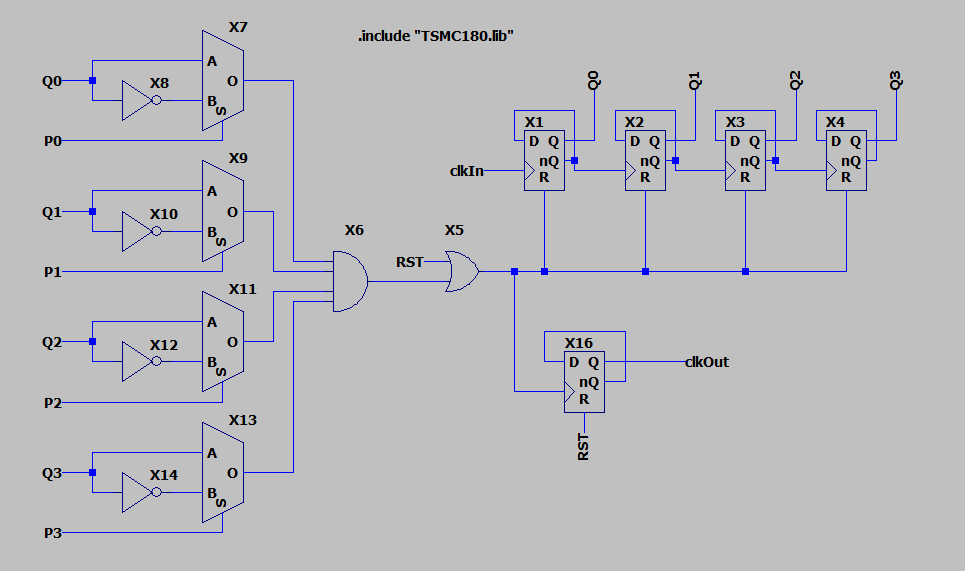
\includegraphics[scale=0.4]{./img/freq_div_2n_v2_sch}
\caption{Divisor de frecuencias de $2N$ con otro comparrador. }
\label{fig:freq_div_2n_v2_sch}
\end{figure}

\begin{figure}[!htb]
\centering
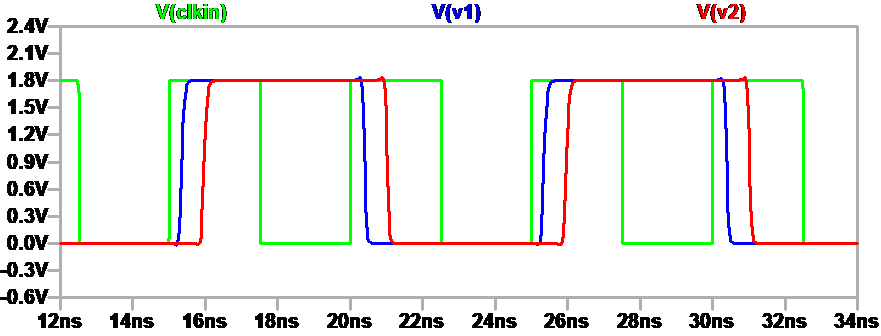
\includegraphics[scale=0.4]{./img/freq_div_2n_test_v1_vs_v2_sim}
\caption{Comparación entre los dos divisores de $2N$. }
\label{fig:freq_div_2n_test_v1_vs_v2_sim}
\end{figure}

Con este divisor de frecuencias, el VCO de la sección anterior y un reloj de entrada de \SI{12}{\mega\hertz}, podríamos producir 11 salidas con frecuencias entre \SI{72}{\mega\hertz} y \SI{312}{\mega\hertz}.

\section{PFD y el Filtro de Lazo}

El PFD (por Phase Frequency Detector) es un componente que toma dos señales y indique la diferencia entre sus fases. Figura \ref{fig:pfd_sch} muestra una implementación de un PFD. En el primer flanco ascendente de  dClock o clkIn la salida de su FFD cambia a un uno. Cuando llega el flanco del otro señal, la salida de su FFD cambia a un uno también, así la salida de la compuerta AND cambia a un uno y pone a cero los dos FFDs. Así la salida UP o DOWN es alto por el tiempo entre los flancos ascendentes de los relojes. Estos dos señales pueden ser combinados en uno para indicar la diferencia en fase. Usando directivos de SPICE medí el tiempo que las señales UP y DOWN estuvieron alto por cada offset entre los relojes entre \SI{-800}{\pico\second} y \SI{800}{\pico\second} en intervales de \SI{10}{\pico\second}, figura \ref{fig:pfd_sim} muestra estas mediciones.

\begin{figure}[!htb]
\centering
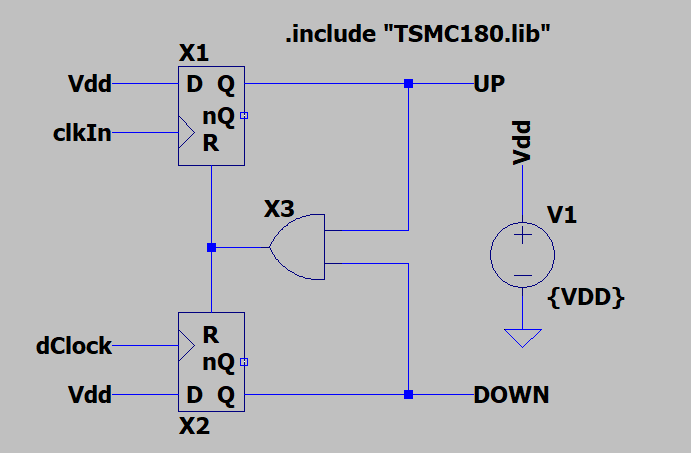
\includegraphics[scale=0.4]{./img/pfd_sch}
\caption{Un PFD básico.}
\label{fig:pfd_sch}
\end{figure}

\begin{figure}[!htb]
\centering
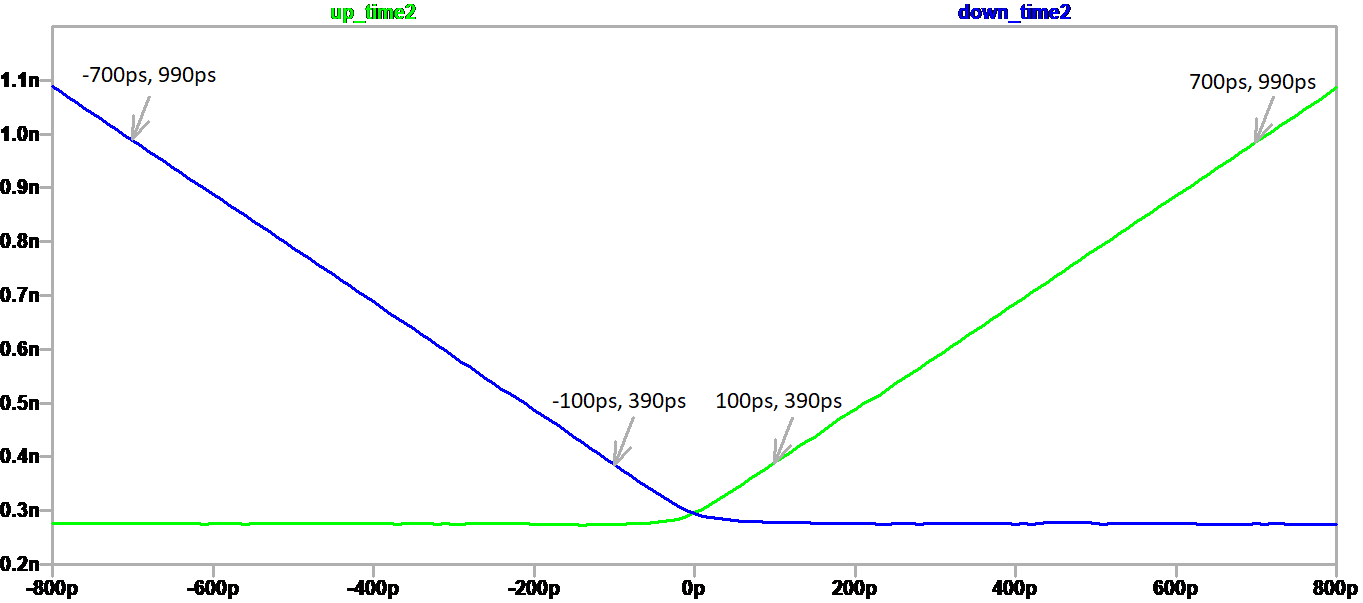
\includegraphics[scale=0.4]{./img/pfd_sim}
\caption{Simulación del PFD básico.}
\label{fig:pfd_sim}
\end{figure}

Figura \ref{fig:pfd_v2_sch} muestra un otro diseño de un PFD, y Figura \ref{fig:pfd_v2_sim} muestra el ancho de los señales UP y DOWN. En este diseño hay un pequeño ``dead zone'' cuándo ninguno de los señales UP y DOWN están altos, pero en el diseño básico hay una superposición de aproximadamente \SI{280}{\pico\second} cuándo los dos señales están altos.
\begin{figure}[!htb]
\centering
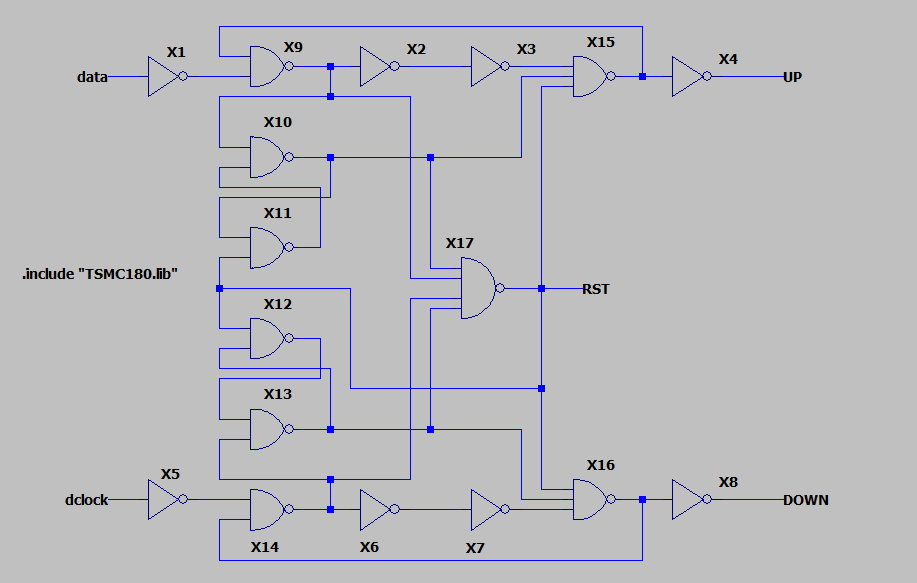
\includegraphics[scale=0.4]{./img/pfd_v2_sch}
\caption{Otro diseño de un PFD.}
\label{fig:pfd_v2_sch}
\end{figure}

\begin{figure}[!htb]
\centering
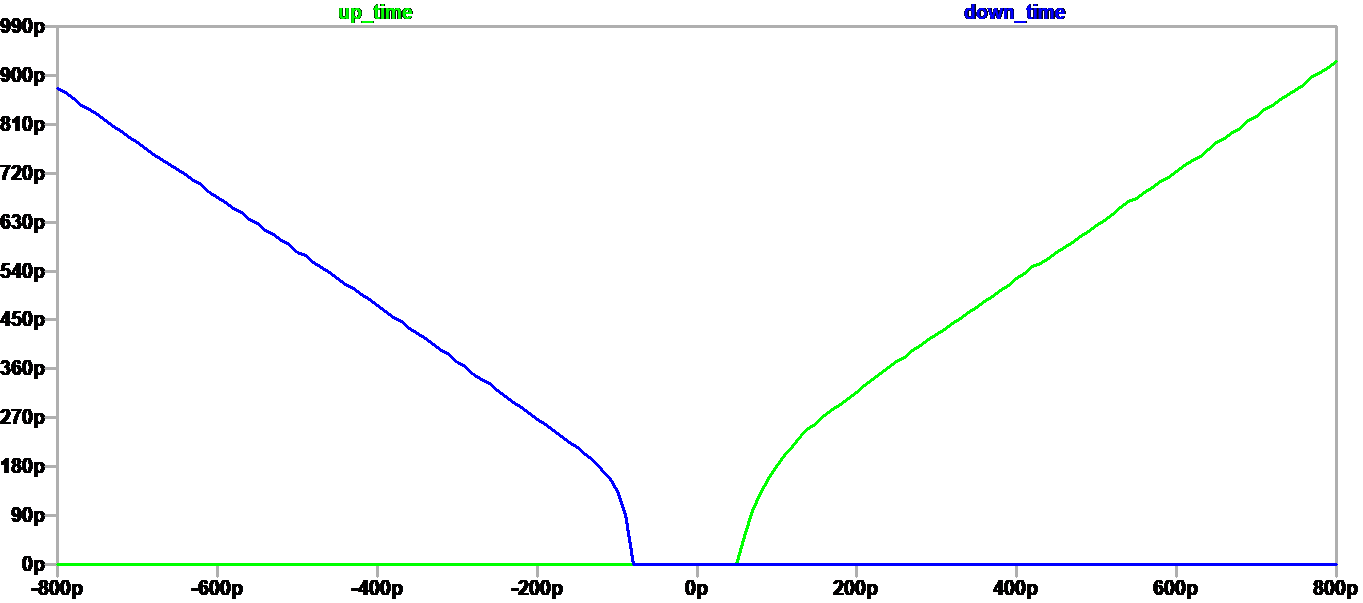
\includegraphics[scale=0.4]{./img/pfd_v2_sim}
\caption{Simulación del otro PFD.}
\label{fig:pfd_v2_sim}
\end{figure}

Para juntar UP y DOWN uso una salida de tri-state, Figura \ref{fig:pfd_tri_state} muestra el esquemático. Cuando UP o DOWN están altos, la carga sobre los drains puede cargar o descargar, pero cuando ninguno de los señales están altos, la salida tiene alta impedancia. El gain del PFD con la salida tri-state es $K_{PD_{tri}} = V_{DD} / 4\pi$.

\begin{figure}[!htb]
\centering
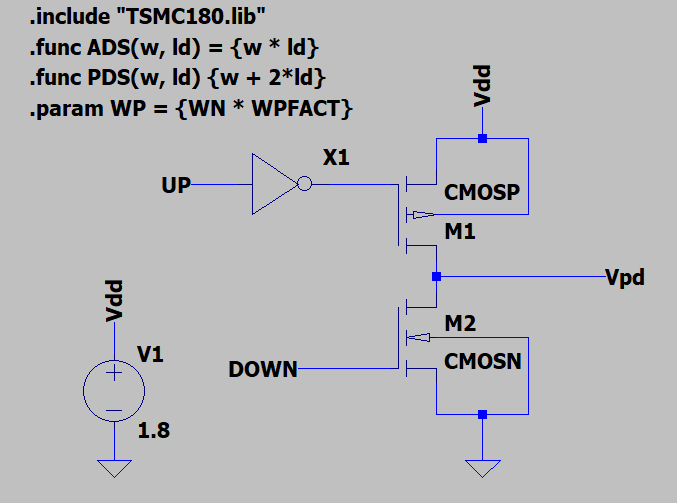
\includegraphics[scale=0.4]{./img/pfd_tri_state}
\caption{Salida de tri-state.}
\label{fig:pfd_tri_state}
\end{figure}

Finalmente es necesario pasar la salida del PFD por un filtro. El filtro usado es mostrado en Figura \ref{fig:pfd_loop_filter_sch}. La función de transferencia del filtro de lazo es: $K_F = \frac{1 + sR_2 C}{s(R_1 + R_2)C}$.

\begin{figure}[!htb]
\centering
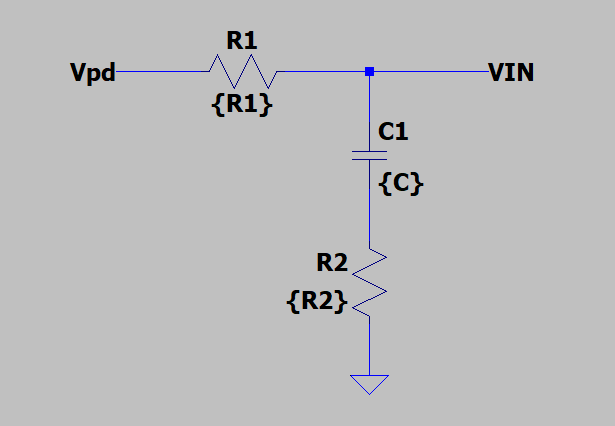
\includegraphics[scale=0.4]{./img/pfd_loop_filter_sch}
\caption{Filtro de Lazo para usar con el PFD con salida tri-state.}
\label{fig:pfd_loop_filter_sch}
\end{figure}

\section{PLLD y Sintetizador de Frecuencias}

Figura \ref{fig:pfd_plld_sch} muestra el esquemático final con todos los componentes conectados. Las ecuaciones para este PLL son:

\begin{align*}
    H(s) &= \frac{K_{PD_{tri}} K_F K_{VCO}}{s + \frac{1}{N} K_{PD_{tri}} K_F K_{VCO}} \\
    \omega_n &= \sqrt{\frac{K_{PD_{tri}} K_{VCO}}{N(R_1 + R_2)C}} \\
    \zeta &= \frac{\omega_n}{2} R_2 C \\
    \Delta\omega_L &= 4\pi\zeta\omega_n \\
    \Delta\omega_P &= \frac{\pi}{2}\sqrt{2\zeta\omega_n K_{VCO} K_{PD_{tri}} - \omega_n^2}
\end{align*}

Donde:
\begin{itemize}[noitemsep]
    \item H(s) = La función de transferencia de fase.
    \item $\omega_n$ = La frecuencia natural.
    \item $\zeta$ = El factor de amortiguamiento.
    \item $\Delta\omega_L$ = El rango de lock.
    \item N = El factor de división.
    \item $\Delta\omega_P$ = El rango de pull-in.
\end{itemize}

Comenzando con $\zeta = 1$, $\Delta\omega_L = \SI{20}{\mega\hertz} \cdot 2\pi$ y $N = 8$. Encontramos $\omega_n = \SI[per-mode=symbol]{10e6}{\radian\per\second}$ y $R_2 C = \SI{200}{\nano\second}$. Eligiendo $C = \SI{10}{\pico\farad}$ y $R_2 = \SI{20}{\kilo\ohm}$, podríamos encontrar $R_1 = \SI{2.56}{\kilo\ohm}$. Porque queremos tener N programable podríamos volver calcular $\omega_n$, $\zeta$, $\Delta\omega_L$, y $\omega_P$ por cada N entre 2 y 30.

\begin{tabular}{| r | r | r | r | r | r | r |} \hline
N   & $\omega_n$ (\SI[per-mode=symbol]{}{\radian\per\second})  & $\zeta$   & $\omega_L$ (\SI[per-mode=symbol]{}{\radian\per\second})  & FL (\SI{}{\mega\hertz}) & Wp (\SI[per-mode=symbol]{}{\radian\per\second})  & Fp (\SI{}{\mega\hertz}) \\ \hline
2   & \SI{20.00E+06}                                        & 2.0       & \SI{503E+06}                                          & 80                    & \SI{521E+06}                                  & 83                    \\
4   & \SI{14.14E+06}                                        & 1.4       & \SI{251E+06}                                          & 40                    & \SI{401E+06}                                  & 64                    \\
6   & \SI{11.55E+06}                                        & 1.2       & \SI{168E+06}                                          & 27                    & \SI{321E+06}                                  & 51                    \\
8   & \SI{10.00E+06}                                        & 1.0       & \SI{126E+06}                                          & 20                    & \SI{270E+06}                                  & 43                    \\
10  & \SI{8.94E+06}                                         & 0.9       & \SI{101E+06}                                          & 16                    & \SI{235E+06}                                  & 37                    \\
12  & \SI{8.16E+06}                                         & 0.8       & \SI{84E+06}                                           & 13                    & \SI{209E+06}                                  & 33                    \\
14  & \SI{7.56E+06}                                         & 0.8       & \SI{72E+06}                                           & 11                    & \SI{189E+06}                                  & 30                    \\
16  & \SI{7.07E+06}                                         & 0.7       & \SI{63E+06}                                           & 10                    & \SI{173E+06}                                  & 27                    \\
18  & \SI{6.67E+06}                                         & 0.7       & \SI{56E+06}                                           & 9                     & \SI{160E+06}                                  & 25                    \\
20  & \SI{6.32E+06}                                         & 0.6       & \SI{50E+06}                                           & 8                     & \SI{149E+06}                                  & 24                    \\
22  & \SI{6.03E+06}                                         & 0.6       & \SI{46E+06}                                           & 7                     & \SI{139E+06}                                  & 22                    \\
24  & \SI{5.77E+06}                                         & 0.6       & \SI{42E+06}                                           & 7                     & \SI{131E+06}                                  & 21                    \\
26  & \SI{5.55E+06}                                         & 0.6       & \SI{39E+06}                                           & 6                     & \SI{124E+06}                                  & 20                    \\
28  & \SI{5.35E+06}                                         & 0.5       & \SI{36E+06}                                           & 6                     & \SI{118E+06}                                  & 19                    \\
30  & \SI{5.16E+06}                                         & 0.5       & \SI{34E+06}                                           & 5                     & \SI{112E+06}                                  & 18                    \\ \hline
\end{tabular}

\begin{figure}[!htb]
\centering
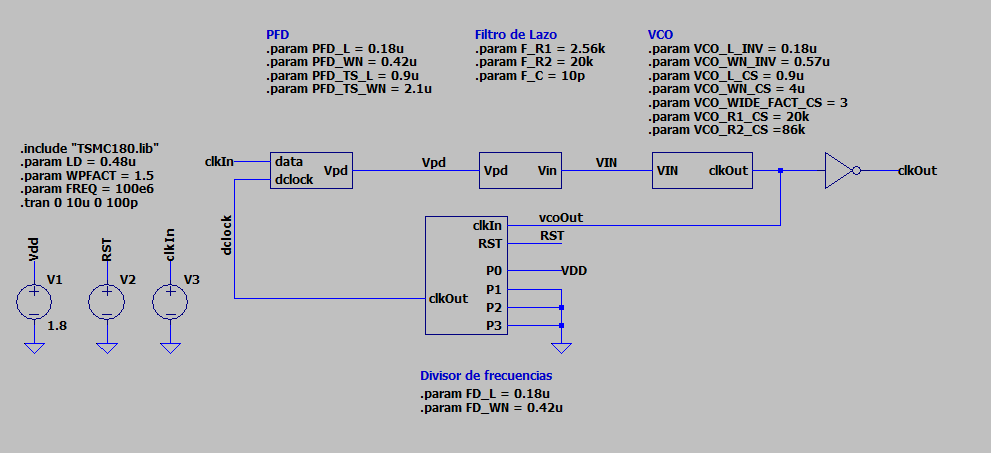
\includegraphics[scale=0.4]{./img/pfd_plld_sch}
\caption{Esquemático del PLLD entero.}
\label{fig:pfd_plld_sch}
\end{figure}

Figuras \ref{fig:pfd_plld_25Min_200Mout}, \ref{fig:pfd_plld_12Min_264Mout}, \ref{fig:pfd_plld_100Min_200Mout} y \ref{fig:pfd_plld_5Min_150Mout} muestran varias simulaciones del PLLD entero con diferentes frecuencias de entrada entre \SI{5}{\mega\hertz} y \SI{100}{\mega\hertz} y diferentes factores de multiplicación entre 2 y 30. Figura \ref{fig:freq_synth_sch} muestra el esquemático de un sintetizador de frecuencias que connsiste en un PLLD, un prescaler y un postscaler. Figurar \ref{fig:freq_synth_100Min_150Mout} muestra una simulación del sintetizador de frecuencias para obtener un reloj de \SI{150}{\mega\hertz} desde un reloj de entrada de \SI{100}{\mega\hertz}.

\begin{figure}[!htb]
\centering
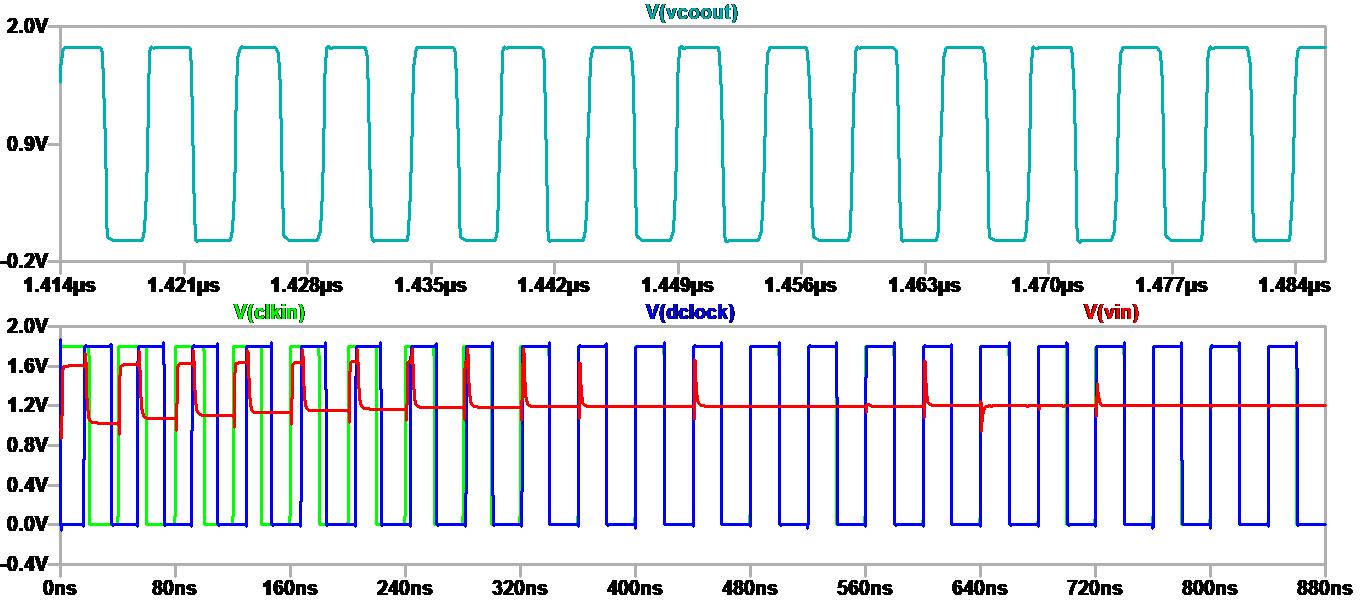
\includegraphics[scale=0.4]{./img/pfd_plld_25Min_200Mout}
\caption{Simulación de un PLLD con reloj de entrada de \SI{25}{\mega\hertz} y salida \SI{200}{\mega\hertz}.}
\label{fig:pfd_plld_25Min_200Mout}
\end{figure}

\begin{figure}[!htb]
\centering
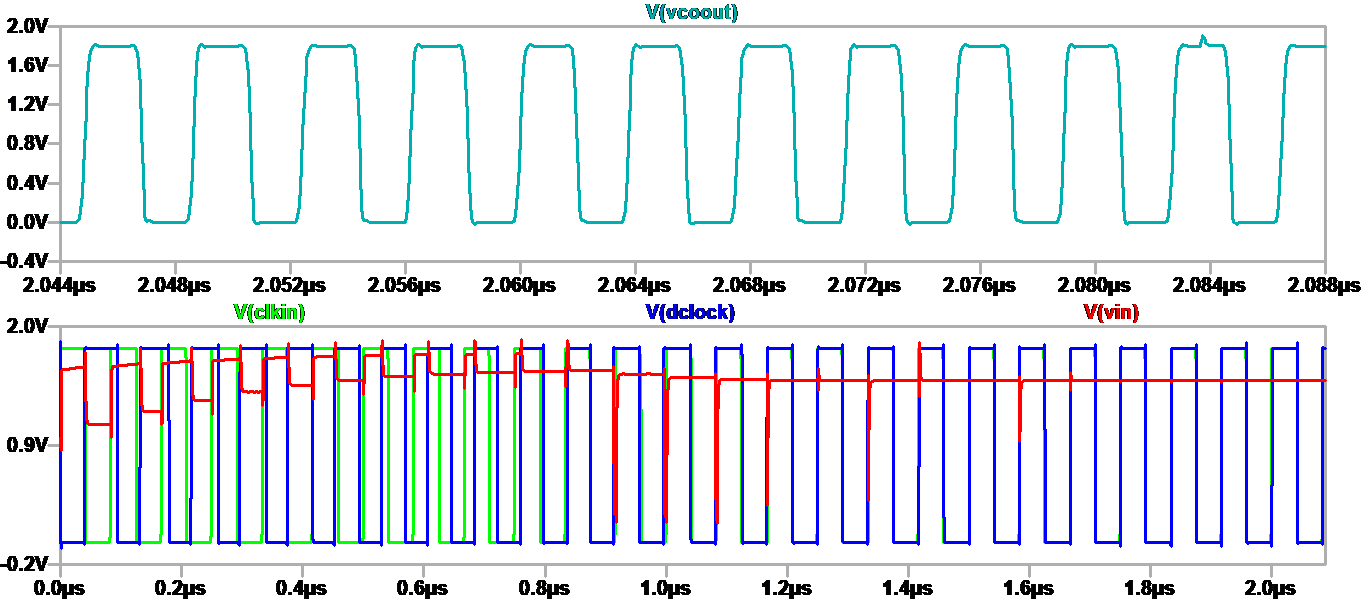
\includegraphics[scale=0.4]{./img/pfd_plld_12Min_264Mout}
\caption{Simulación de un PLLD con reloj de entrada de \SI{12}{\mega\hertz} y salida \SI{264}{\mega\hertz}.}
\label{fig:pfd_plld_12Min_264Mout}
\end{figure}

\begin{figure}[!htb]
\centering
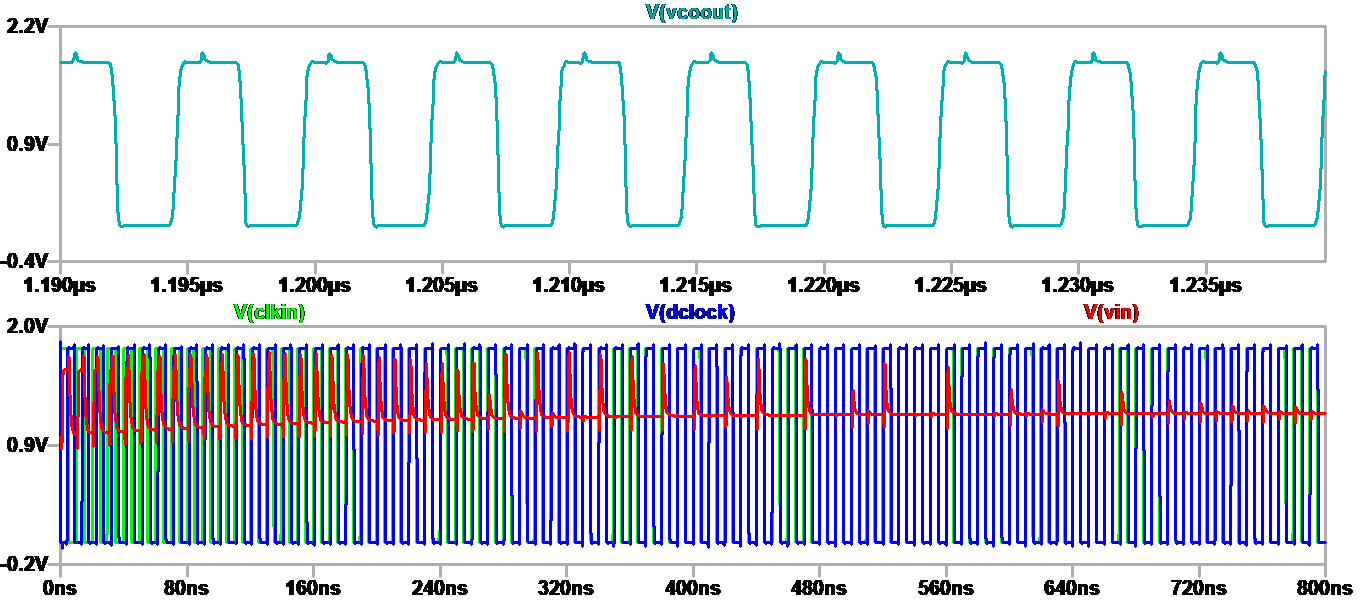
\includegraphics[scale=0.4]{./img/pfd_plld_100Min_200Mout}
\caption{Simulación de un PLLD con reloj de entrada de \SI{100}{\mega\hertz} y salida \SI{200}{\mega\hertz}.}
\label{fig:pfd_plld_100Min_200Mout}
\end{figure}

\begin{figure}[!htb]
\centering
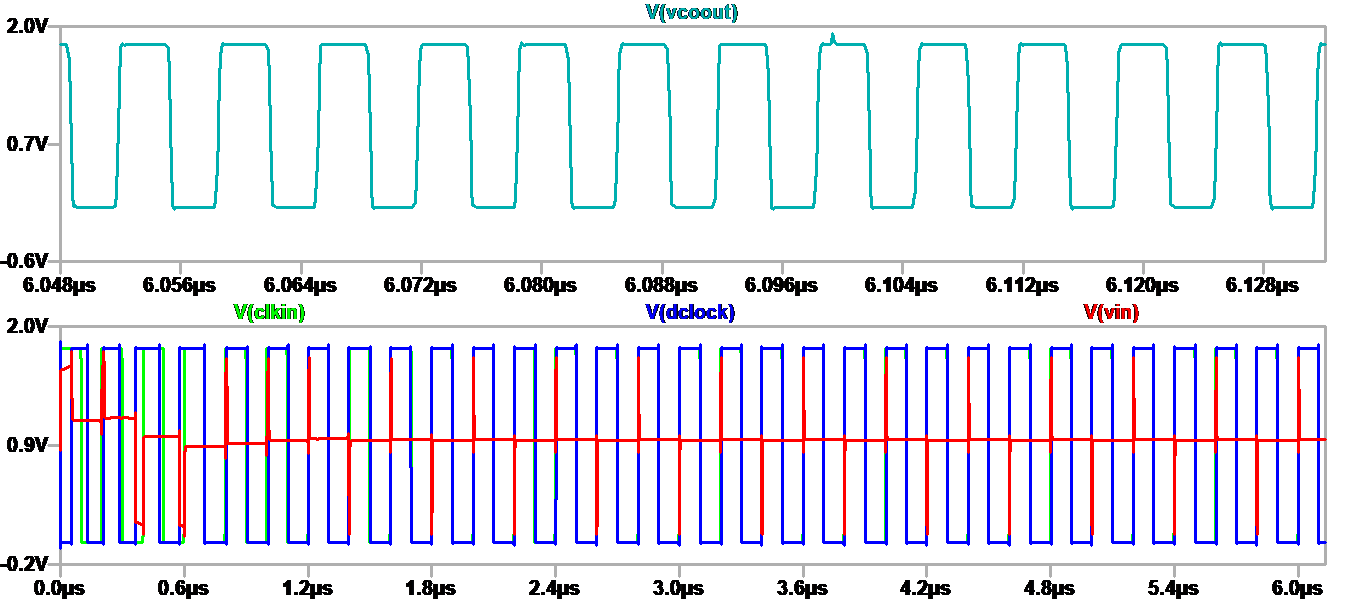
\includegraphics[scale=0.4]{./img/pfd_plld_5Min_150Mout}
\caption{Simulación de un PLLD con reloj de entrada de \SI{5}{\mega\hertz} y salida \SI{150}{\mega\hertz}.}
\label{fig:pfd_plld_5Min_150Mout}
\end{figure}

\begin{figure}[!htb]
\centering
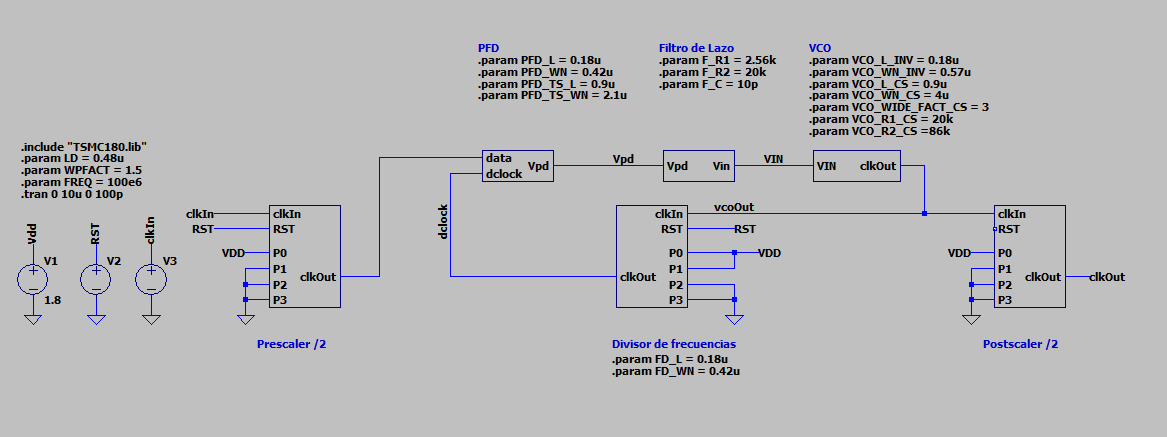
\includegraphics[scale=0.4]{./img/freq_synth_sch}
\caption{Esquemático de un sintetizador de frecuencias.}
\label{fig:freq_synth_sch}
\end{figure}

\begin{figure}[!htb]
\centering
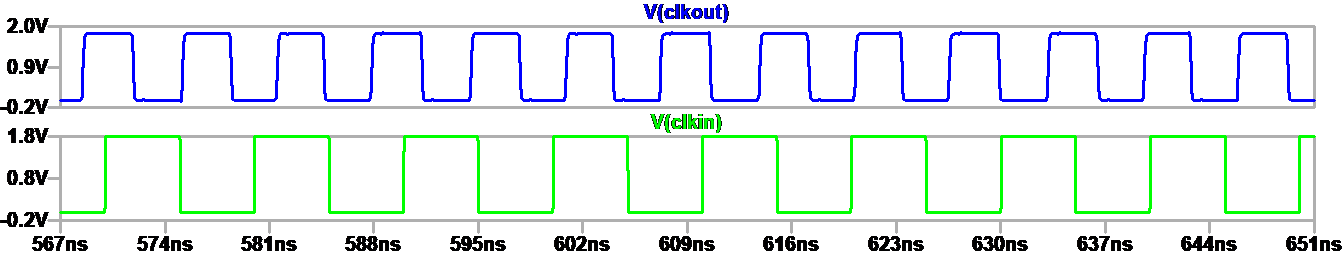
\includegraphics[scale=0.4]{./img/freq_synth_100Min_150Mout}
\caption{Simulación de un sintetizador de frecuencias con reloj de entrada de \SI{100}{\mega\hertz} y salida \SI{150}{\mega\hertz}.}
\label{fig:freq_synth_100Min_150Mout}
\end{figure}

\begin{thebibliography}{9}

\bibitem{RBaker}
R. Jacob Baker (2010) \emph{CMOS: Circuit design, layout and simulation}, Wiley-IEEE Press, 3rd edition.

\bibitem{vco}
Suman, Shruti \& G Sharma, K \& Ghosh, Pradip. (2016). \emph{Analysis and Design of Current Starved Ring VCO}. 10.1109/ICEEOT.2016.7755299.

\bibitem{high_speed_pll}
Rushabh Mehta (2016) \emph{Ddesign and Implementation of a phase locked loop for high-speed serial links}. University of Illinois. \url{http://emlab.uiuc.edu/jose/Theses/mehta_ms.pdf}.

\bibitem{filters}
\emph{Passive Filters}. \url{http://aries.ucsd.edu/najmabadi/CLASS/ECE60L/02-S/NOTES/filter.pdf}.

\end{thebibliography}

\end{document}